\chapter{Business Process Modeling}\label{ch-08}

\lecturemeta{Capitolo originale: 8 --- Business Process Modeling \quad\textbullet\quad Antonio Brogi}{Appunti di Emiliano Sescu (github.com/Faxatos), cap. 8}

Il \textbf{Business Process Management} (BPM) è il metodo sistematico
con cui si analizzano i processi di business esistenti di
un'organizzazione e si introducono miglioramenti per rendere il flusso
di lavoro più efficace ed efficiente (IBM ci ha fatto una fortuna).

\begin{boxdefinition}{Processo, modello, istanza}

\begin{itemize}
\tightlist
\item
  Un \textbf{processo di business} è un insieme di attività di business
  che rappresentano i passi necessari per raggiungere un obiettivo di
  business.
\item
  Un \textbf{modello di processo} (Fig. 8.1) è formato da un insieme di
  modelli di attività e dai \textbf{vincoli di esecuzione} tra di esse.
\item
  Un'\textbf{istanza di processo} è un caso concreto nell'operatività di
  un'azienda, formato da istanze di attività.
\end{itemize}

\end{boxdefinition}

\begin{figure}[H]
\centering
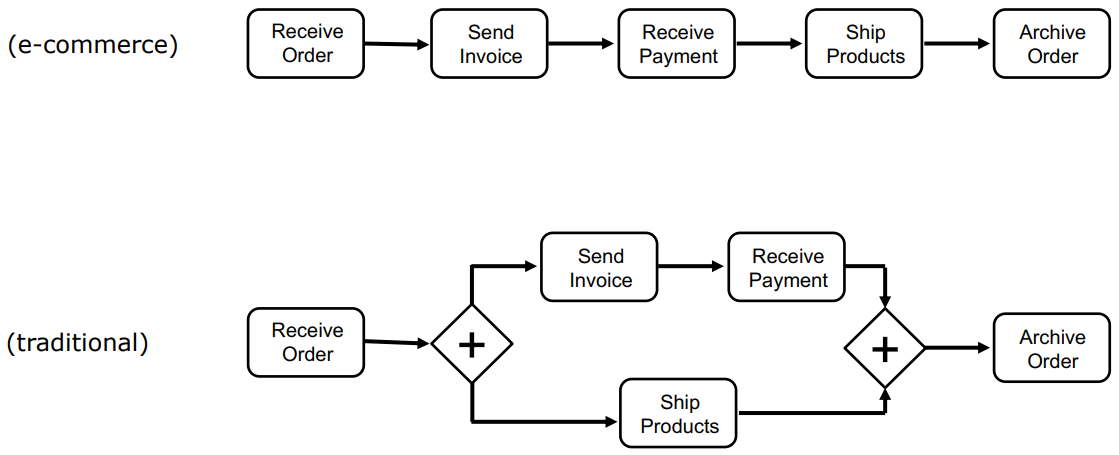
\includegraphics[width=1.00\linewidth,height=0.45\textheight,keepaspectratio]{images/08-bpm_fig8-1_modello-processo.png}
\caption{Esempio di modello di processo di business.}
\end{figure}

\section{BPMN}\label{bpmn}

La \textbf{Business Process Model and Notation (BPMN)} è la notazione
grafica standard per modellare i processi di business (Fig. 8.2).

\begin{figure}[H]
\centering
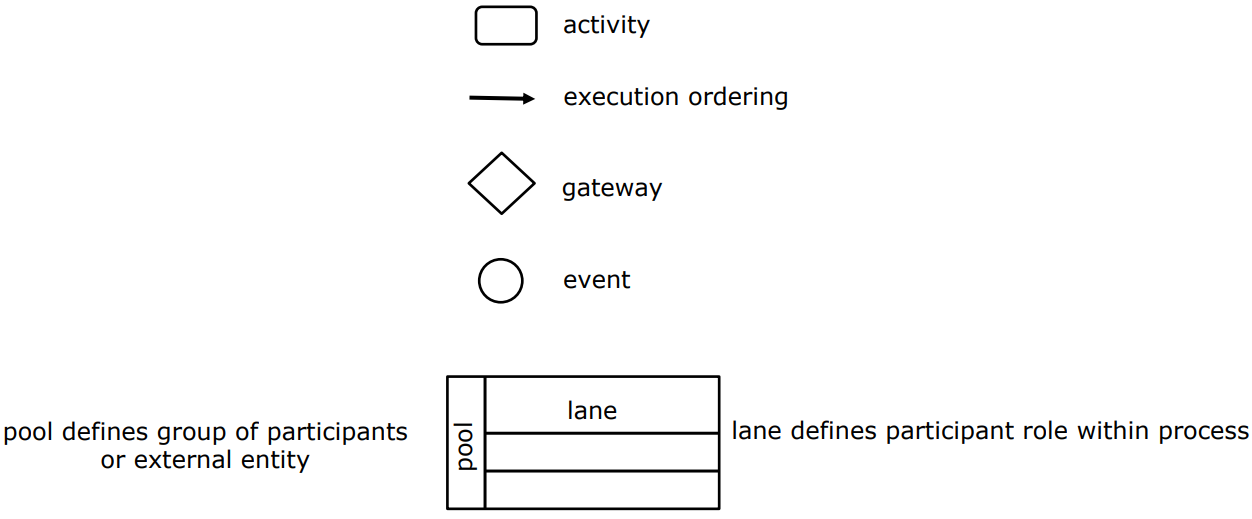
\includegraphics[width=1.00\linewidth,height=0.45\textheight,keepaspectratio]{images/08-bpm_fig8-2_notazione-bpmn.png}
\caption{La notazione grafica per il business process modeling.}
\end{figure}

La Fig. 8.3 mostra un esempio completo, con il funzionamento di tre tipi
di \textbf{gateway}:

\begin{itemize}
\tightlist
\item
  \textbf{parallelo} (AND): attiva tutti i rami in uscita e, in
  ingresso, aspetta che arrivino tutti;
\item
  \textbf{esclusivo} (XOR): sceglie \textbf{uno solo} dei rami in
  uscita;
\item
  \textbf{inclusivo} (OR): attiva \textbf{uno o più} rami in base a una
  condizione su ciascuno; in ingresso aspetta tutti i rami che erano
  stati attivati.
\end{itemize}

\begin{figure}[H]
\centering
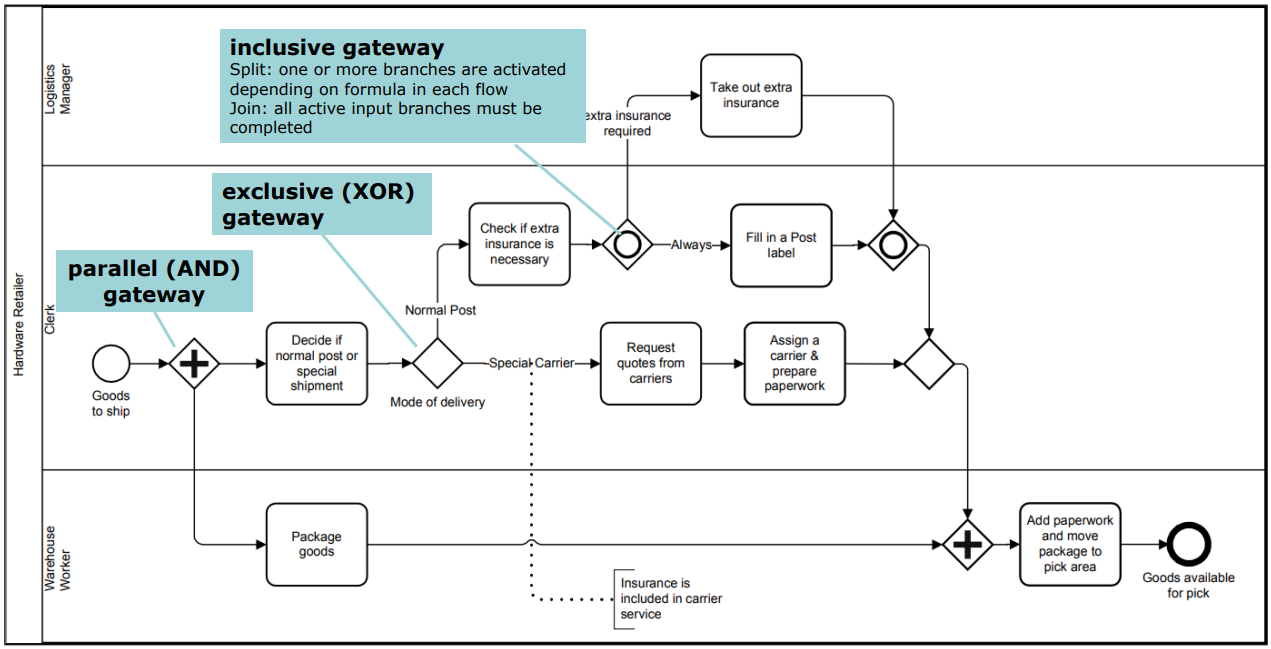
\includegraphics[width=1.00\linewidth,height=0.45\textheight,keepaspectratio]{images/08-bpm_fig8-3_spedizione-hardware.png}
\caption{Esempio: processo di spedizione di un rivenditore di hardware.}
\end{figure}

La Fig. 8.4 mostra come più processi possono interagire tramite
\textbf{message flow} (frecce tratteggiate tra pool diversi). C'è un
processo principale e uno secondario. Quando si raggiunge un
\textbf{terminate event}, tutte le attività del processo terminano
subito. Nel processo principale si vedono anche un \textbf{timer event}
e un \textbf{event-based gateway} (che aspetta un evento per scegliere
il ramo).

\begin{figure}[H]
\centering
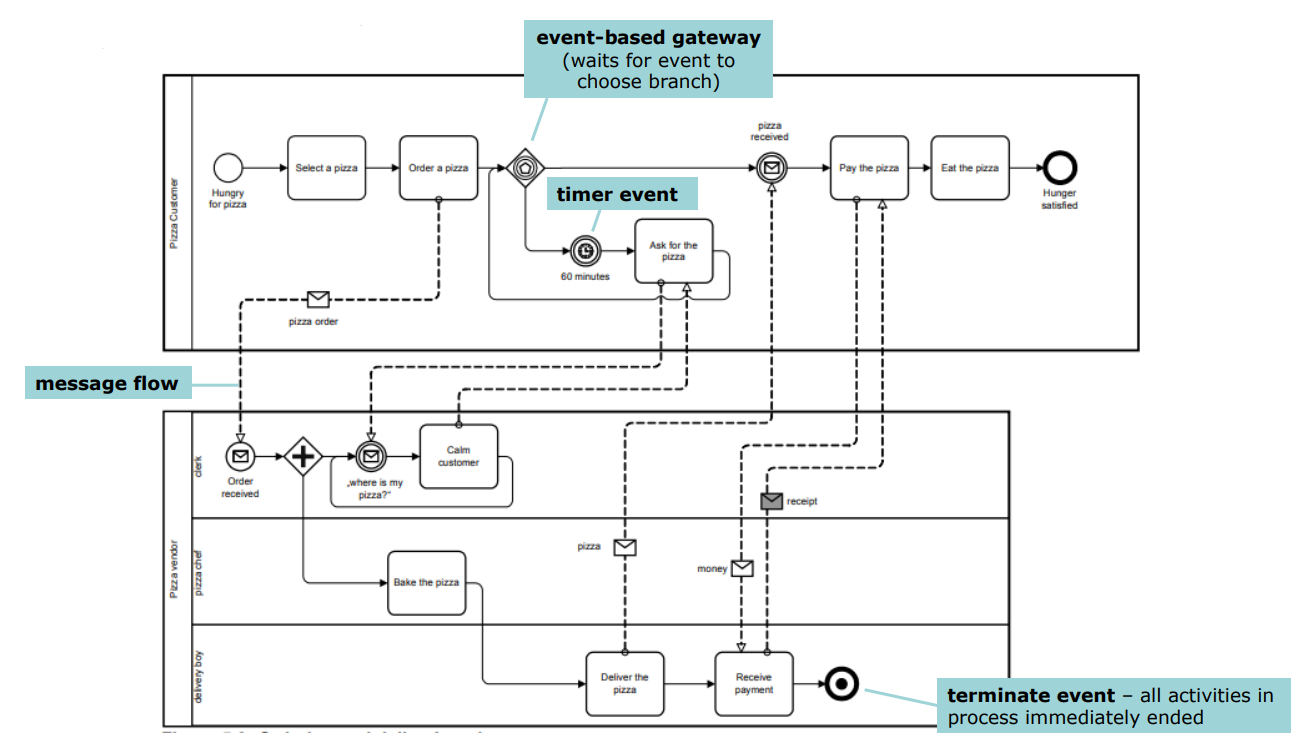
\includegraphics[width=1.00\linewidth,height=0.45\textheight,keepaspectratio]{images/08-bpm_fig8-4_collaborazione-pizza.png}
\caption{Esempio di collaborazione B2B (pizza).}
\end{figure}

L'ultimo esempio (Fig. 8.5) mostra la notazione dei
\textbf{sotto-processi} (\emph{sub-process}) e degli \textbf{eventi
agganciati} (\emph{attached event}) al bordo di un'attività:

\begin{itemize}
\tightlist
\item
  \textbf{error} → \textbf{interrompente}: se scatta, l'attività viene
  interrotta e si segue il ramo dell'evento;
\item
  \textbf{escalation} → \textbf{non interrompente}: se scatta, si avvia
  il ramo dell'evento ma l'attività continua.
\end{itemize}

\begin{figure}[H]
\centering
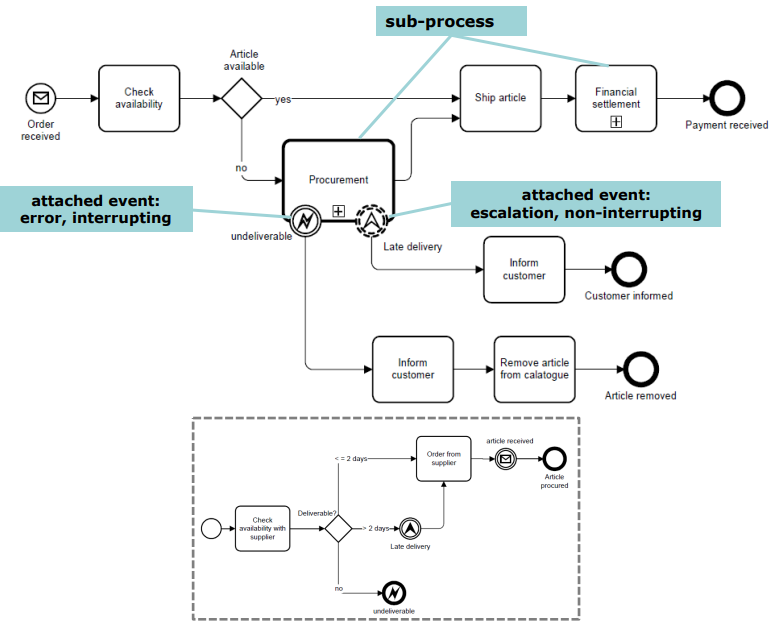
\includegraphics[width=1.00\linewidth,height=0.45\textheight,keepaspectratio]{images/08-bpm_fig8-5_order-fulfillment.png}
\caption{Esempio: evasione dell'ordine e approvvigionamento.}
\end{figure}

\begin{boxnote}{Collegamento con il corso di BPM}

BPMN, reti di Petri e soundness sono trattati in dettaglio negli appunti
di Business Process Modeling: \href{07a\%20-\%20EPC\%20e\%20BPMN}{07a -
EPC e BPMN}, \href{04\%20-\%20Petri\%20Nets}{04 - Petri Nets},
\href{12\%20-\%20Soundness}{12 - Soundness}.

\end{boxnote}

\section{Workflow net}\label{workflow-net}

Nel BPM è fondamentale poter \textbf{dimostrare proprietà} dei modelli
di processo.

Le \textbf{workflow net} sono un'estensione delle \textbf{reti di Petri}
e sono una delle tecniche più note per specificare processi di business
in modo \textbf{formale e astratto}. La rappresentazione grafica delle
reti di Petri facilita la comunicazione tra stakeholder diversi, e le
proprietà del processo si possono analizzare formalmente con vari
strumenti disponibili.

La Fig. 8.6 mostra come una rete di Petri renda leggibile un modello di
processo, traducendo l'esempio di Fig. 8.1.

\begin{figure}[H]
\centering
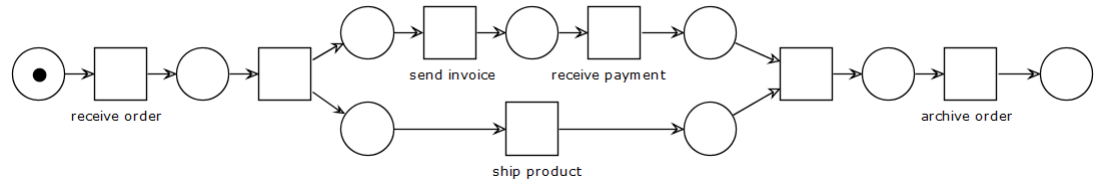
\includegraphics[width=1.00\linewidth,height=0.45\textheight,keepaspectratio]{images/08-bpm_fig8-6_rete-petri-esempio.png}
\caption{La rete di Petri dell'esempio precedente (Fig. 8.1).}
\end{figure}

\subsection{Reti di Petri}\label{reti-di-petri}

Una \textbf{rete di Petri} è formata da:

\begin{itemize}
\tightlist
\item
  \textbf{transizioni} (quadrati), che modellano le \textbf{attività};
\item
  \textbf{posti} (\emph{place}, cerchi) e \textbf{archi} orientati tra
  posti e transizioni, che modellano i \textbf{vincoli di esecuzione}.
\end{itemize}

La dinamica del sistema è rappresentata dai \textbf{token} (i pallini):
come sono distribuiti nei posti determina lo \textbf{stato} del sistema
modellato.

\begin{boxdefinition}{Regola di scatto}

\begin{itemize}
\tightlist
\item
  Una transizione \textbf{può scattare} (è \emph{abilitata}) se c'è
  \textbf{un token in ognuno dei suoi posti di input} (Fig. 8.7).
\item
  Quando scatta, \textbf{toglie un token} da ogni posto di input e
  \textbf{aggiunge un token} a ogni posto di output (Fig. 8.8).
\end{itemize}

\end{boxdefinition}

\begin{figure}[H]
\centering
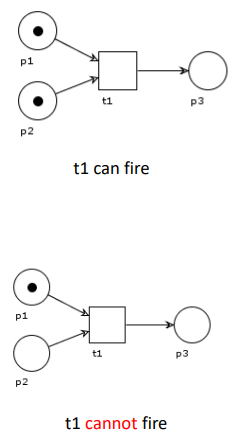
\includegraphics[width=0.30\linewidth,height=0.45\textheight,keepaspectratio]{images/08-bpm_fig8-7_regola-input.png}
\caption{Reti di Petri: la regola di input.}
\end{figure}

\begin{figure}[H]
\centering
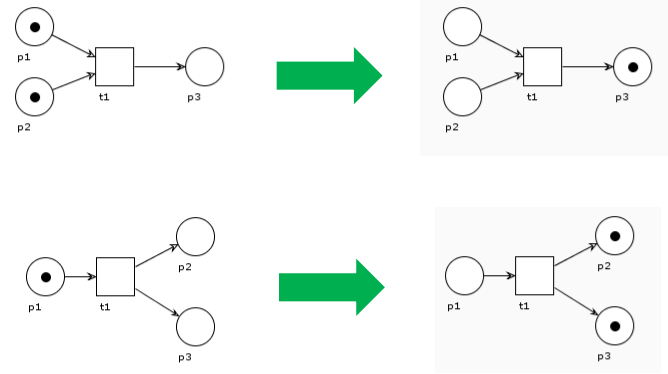
\includegraphics[width=0.80\linewidth,height=0.45\textheight,keepaspectratio]{images/08-bpm_fig8-8_regola-output.png}
\caption{Reti di Petri: la regola di output.}
\end{figure}

\subsection{Workflow net e soundness}\label{workflow-net-e-soundness}

Le workflow net arricchiscono le reti di Petri con notazioni che
semplificano la rappresentazione dei processi di business. Come le reti
di Petri, si concentrano sul \textbf{flusso di controllo} del processo:

\begin{itemize}
\tightlist
\item
  le \textbf{transizioni} rappresentano le \textbf{attività};
\item
  i \textbf{posti} rappresentano le \textbf{condizioni};
\item
  i \textbf{token} rappresentano le \textbf{istanze di processo}.
\end{itemize}

La Fig. 8.9 mostra alcuni pattern di composizione utilizzabili con le
reti di Petri.

\begin{boxdefinition}{Workflow net}

Una rete di Petri è una \textbf{workflow net} se e solo se:

\begin{enumerate}
\def\labelenumi{\arabic{enumi}.}
\tightlist
\item
  c'è un \textbf{unico posto sorgente} (\emph{source}, \(i\)) senza
  archi in ingresso;
\item
  c'è un \textbf{unico posto pozzo} (\emph{sink}, \(o\)) senza archi in
  uscita;
\item
  ogni posto e ogni transizione si trova su \textbf{qualche cammino} dal
  posto iniziale a quello finale.
\end{enumerate}

\end{boxdefinition}

\begin{boxdefinition}{Soundness}

Una workflow net è \textbf{sound} (corretta) se e solo se:

\begin{enumerate}
\def\labelenumi{\arabic{enumi}.}
\tightlist
\item
  ogni esecuzione della rete che parte dallo stato iniziale (un token
  nel posto sorgente, nessun altro token) \textbf{arriva prima o poi
  allo stato finale} (un token nel posto pozzo, nessun altro token);
\item
  ogni transizione compare in \textbf{almeno un'esecuzione} della rete.
\end{enumerate}

\end{boxdefinition}

\begin{boxwarning}{Cosa dice (e cosa non dice) la soundness}

Le workflow net \textbf{astraggono dai dati}: le scelte che dipendono
dai dati diventano scelte ``alla cieca''. Di conseguenza l'analisi può
considerare \textbf{più rami del necessario}.

\begin{itemize}
\tightlist
\item
  Una rete \textbf{non sound} va presa solo come un
  \textbf{avvertimento} di possibili problemi a runtime: l'analisi di un
  ramo che in realtà non verrà mai eseguito può rendere la rete non
  sound, anche se l'applicazione non lo eseguirà mai.
\item
  Al contrario, l'analisi di un ciclo può non accorgersi che
  l'applicazione non terminerà mai: una rete \textbf{sound non
  garantisce} che l'applicazione termini sempre.
\end{itemize}

\end{boxwarning}

\begin{figure}[H]
\centering
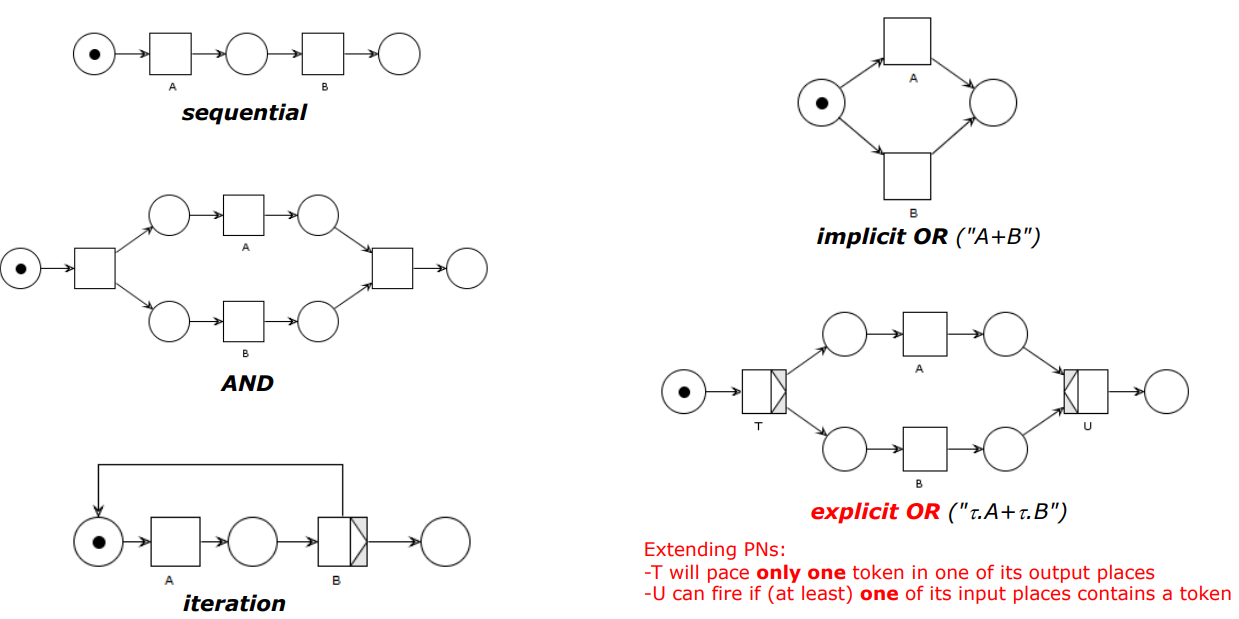
\includegraphics[width=0.97\linewidth,height=0.45\textheight,keepaspectratio]{images/08-bpm_fig8-9_pattern-composizione.png}
\caption{Pattern di composizione delle reti di Petri.}
\end{figure}

\subsection{Verificare la soundness}\label{verificare-la-soundness}

Come si stabilisce in modo formale (e automatico) se una rete è sound?
Servono prima due proprietà:

\begin{boxdefinition}{Liveness}

Una rete di Petri \((PN, M)\) è \textbf{viva} (\emph{live}) se e solo se
per ogni stato raggiungibile \(M'\) e per ogni transizione \(t\) esiste
uno stato \(M''\) raggiungibile da \(M'\) in cui \(t\) è abilitata.

In parole semplici: da qualunque punto si arrivi, ogni transizione può
ancora scattare prima o poi.

\end{boxdefinition}

\begin{figure}[H]
\centering
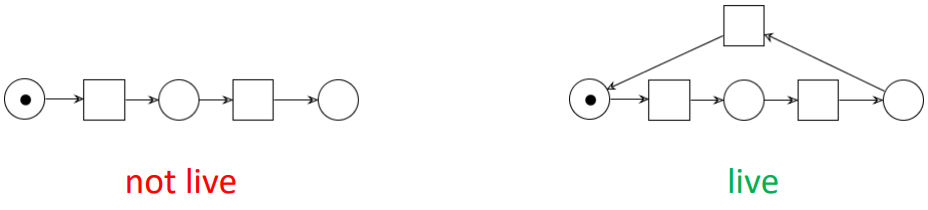
\includegraphics[width=0.69\linewidth,height=0.45\textheight,keepaspectratio]{images/08-bpm_esempio-live.png}
\caption*{Esempio di rete non viva (a sinistra) e viva (a destra).}
\end{figure}

\begin{boxdefinition}{Boundedness}

Una rete di Petri \((PN, M)\) è \textbf{limitata} (\emph{bounded}) se e
solo se per ogni posto \(p\) esiste un \(n \in \mathbb{N}\) tale che, in
ogni stato raggiungibile \(M'\), il numero di token in \(p\) è minore di
\(n\).

In parole semplici: nessun posto può accumulare infiniti token.

\end{boxdefinition}

\begin{figure}[H]
\centering
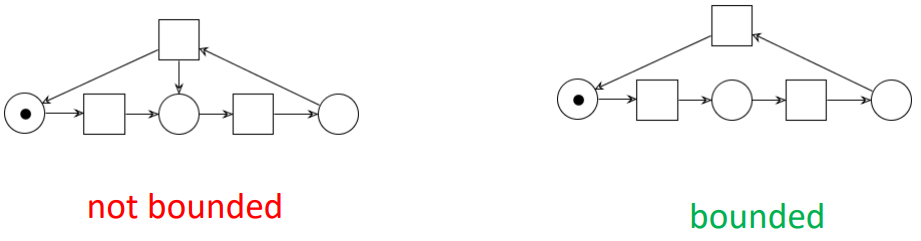
\includegraphics[width=0.69\linewidth,height=0.45\textheight,keepaspectratio]{images/08-bpm_esempio-bounded.png}
\caption*{Esempio di rete non limitata (a sinistra) e limitata (a destra).}
\end{figure}

\begin{boxtheorem}{Soundness tramite liveness e boundedness}

Una workflow net \(N\) è \textbf{sound} se e solo se
\((\overline{N}, \{i\})\) è \textbf{viva e limitata}, dove
\(\overline{N}\) è la rete \(N\) a cui si aggiunge una transizione che
va dal posto pozzo \(o\) al posto sorgente \(i\).

\end{boxtheorem}

\begin{boxtip}{Perché si aggiunge la transizione da \(o\) a \(i\)}

``Cortocircuitando'' la rete, il processo può ripartire dopo aver
finito. Così la domanda ``ogni esecuzione termina correttamente e ogni
attività è utile?'' diventa una domanda su proprietà classiche (liveness
e boundedness) che i tool sanno già verificare.

\end{boxtip}
